\documentclass[a4paper,oneside,12pt]{article}

%\usepackage{natbib}

\usepackage[utf8]{inputenc}
\usepackage[T1]{fontenc}
\usepackage[english]{babel}


% Packages
\usepackage{amsmath,amsfonts,amssymb,amsopn,amscd,amsthm}
\usepackage{comment}
\usepackage{dsfont}
\usepackage{graphicx,float}
\usepackage{color}
\usepackage[colorlinks]{hyperref}
\usepackage{epigraph}
\usepackage{todonotes}
\usepackage[left=2cm,top=2cm,bottom=2cm,right=2cm]{geometry}
\usepackage{tikz-cd}
\usepackage{caption}
\usepackage{subcaption}

\hypersetup{
  colorlinks,
  citecolor=blue,
  linkcolor=red
}



\DeclareCaptionFormat{custom}
{%
    \textbf{#1#2}\textit{\small #3}
}
\captionsetup{format=custom}

%\usepackage{geometry}
%\usepackage{enumitem}
%\usepackage[babel]{csquotes}
%\usepackage{graphicx}
\usepackage{bbm}
%\usepackage{tikz}
%\usepackage{pgfplots}
%\usepackage{dsfont}
\usepackage{faktor}
%\usepackage{amsthm}
\usepackage{cancel}
\usepackage{indentfirst}
%\usepackage{comment}
\usepackage{stmaryrd}
%\MakeAutoQuote{«}{»}
%\geometry{dvips,a4paper,hmargin=2cm,vmargin=2.5cm}


\theoremstyle{plain}
\newtheorem{theorem}{Theorem}[section]
\newtheorem{corollary}[theorem]{Corollary}
\newtheorem{prop}[theorem]{Proposition}
\newtheorem{lemma}[theorem]{Lemma}
\newtheorem{definition}{Definition}[section]
\newtheorem{assumption}[definition]{Assumption}
\newtheorem*{remark}{Remarque}
\newtheorem*{ex}{Example}

%\numberwithin{algorithm}{section}
% \numberwithin{equation}{section}
% \numberwithin{figure}{section}
% \numberwithin{table}{section}

\usepackage{pstricks,pstricks-add,pst-node,pst-tree}
%\pgfplotsset{compat=1.16}


\title{TD2 - L2 BCP}
\author{}
\date{}

%Ordinals
\def\N{{\mathbb N}}
\def\Z{{\mathbb Z}}
\def\Q{{\mathbb Q}}
\def\R{{\mathbb R}}
\def\C{{\mathbb C}}
\def\H{{\mathbb H}}
\def\S{{\mathbb S}}
\def\T{{\mathbb T}}
\def\K{{\mathbb K}}
\def\W{\mathbb{W}}
\def\D{\mathbb{D}}
\def\V{\mathbb{V}}

%Probability
\def\P{{\mathbb P}}
\def\E{{\mathbb E}}
\def\F{{\mathbb F}}
\def\X{{\mathbb X}}
\def\Y{{\mathbb Y}}
\def\F{{\mathcal F}}
\def\U{{\mathcal U}}
\def\Cov{{\mbox Cov}}

%Index
\def\u{{\textbf{u}}}
\def\v{{\textbf{v}}}




\begin{document}



\maketitle

\section*{Exercice 1}

Ici on note $X \sim \mathcal{N}(\mu; \sigma)$ le poids en gramme d'une larve prise au hasard, où $\mu = 3g$ et $\sigma = 0,42g$.

\begin{enumerate}
    \item $X$ est une variable continue, donc, :
    $$\forall a \in \R,\; \P(X=a) = 0$$
    En particulier $\P(X=3) = 0$.
    \item Il y a reproduction si le poids est supérieur à la moyenne $\mu = 3,4 g$. On se ramène donc à calculer $\P(X>\mu)$. Mais X étant une variable suivant une loi normale \textbf{sa médiane est sa moyenne}. Par définition de la médiane : $\P(X> \mu) = 0,5$.
    \begin{remark}
    On note que $\P(X> \mu) = \P(X\ge \mu)$, grâce à la même propriété des variables continues utilisée en question 1.
    \end{remark}
    \item Dans l'idée d'utiliser la 1.4.1 du polycopié de cours, posons $$X_0 = \frac{X-\mu}{\sigma}\sim\mathcal{N}(0; 1)$$
    On connaît donc les valeurs de la fonction de répartition de $X_0$, grâce aux tables. Calculons la probabilité demandée :
    \begin{align*}
        \P(X<3,75)&=\P\left(X-\mu<3,75-\mu\right)\\
        &=\P\left(\frac{X-\mu}{\sigma}<\frac{3,75-\mu}{\sigma}\right)\\
        &=\P(X_0<0,833) \qquad \qquad \left( \mbox{car } \frac{3,75-\mu}{\sigma} = \frac{3,75-3,4}{0,42} = 0,833\right)\\
        &= 79,67\% \qquad \qquad \mbox{(d'après les tables)}
    \end{align*}
    \item Notons ici que l'utilisation du terme "proportion" fait évidemment référence au calcul de la probabilité correspondante.
    Commençons par nous ramener au calcul de la probabilité de la variable centrée réduite. 
    \begin{align*}
        \P(X>3)&=\P\left(X-\mu>3-\mu\right)\\
        &=\P\left(\frac{X-\mu}{\sigma}>\frac{3-\mu}{\sigma}\right)\\
        &=\P(X_0>-0,95) \qquad \qquad \left( \mbox{car } \frac{3-\mu}{\sigma} = \frac{3-3,4}{0,42} =- 0,95\right)\\
    \end{align*}
    Pour se ramener à la fonction de répartition (dont les valeurs sont données par les tables), on pourrait se ramener à regarder la probabilité du complémentaire :$$ \P(X_0>-0,95) = 1 - \P(X_0<-0,95)$$
    mais les tables ne donnent les valeurs de la fonction de répartition que pour des valeurs de $x$ positives. On va donc utiliser la symétrie de la loi normale (remarque en haut de la page 12 du polycopié de cours) :
    $$\P(X_0>-0,95) = \P(X_0<0,95)$$
    De façon générale on a $$\forall a \in \R,\; \P(X_0>-a) = \P(X_0<a)$$
    visible en faisant un dessin.
    
    On peut conclure avec les tables:
    $$\P(X>3) = \P(X_0<0,95) = 82,89\%$$
    
    \item Voici une esquisse de la densité :
    \begin{figure}[h]
    \centering
    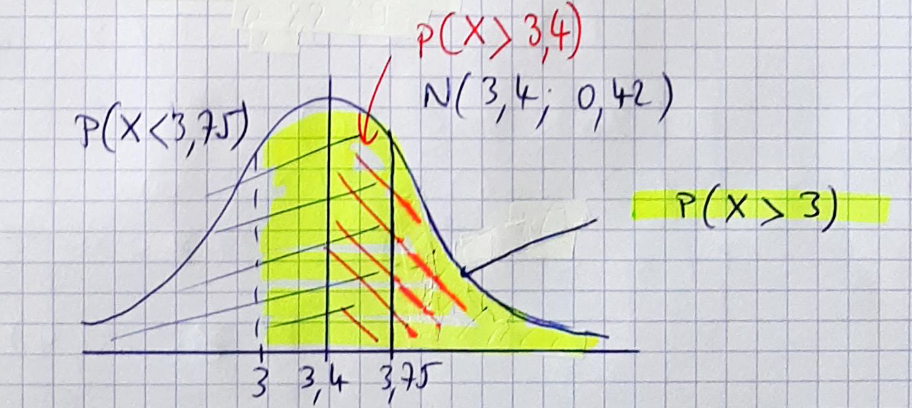
\includegraphics[width = \textwidth]{images/question_5.png}
\end{figure}

    \item Ici, l'idée va être d'utiliser une variante de la proposition 1.4.2 du cours. En effet, commençons par raisonner sur la façon de modéliser notre problème. On observe le poids de 50 larves prises au hasard, de façon indépendante d'après l'exercice. C'est pourquoi on va se ramener à modéliser $Z$ par :
    $$Z = X_1 + \dots X_{50}$$ 
    où chaque $X_i \sim \mathcal{N}(\mu; \sigma)$ sera indépendante des autres.
    Maintenant que nous avons modéliser notre problème, regardons les outils mathématiques à notre disposition. Si on regarde la propriété 1.4.2 pour $\alpha = \beta = 1$, on a 
    $$X_1 + X_2 \sim \mathcal{N}(\mu +\mu; \sqrt{\sigma^2 + \sigma^2}) =\mathcal{N}(2\mu; \sqrt{2\sigma^2}) $$
    En raisonnant par récurrence, on peut généraliser le précédent résultat à :
    $$Z = X_1 + \dots X_{50} \sim\mathcal{N}(50\mu; \sqrt{50\sigma^2})$$
    


    Cette propriété peut être admise (cf. dernière ligne des diapositives du chapitre 2 - diapo 22/24), mais l'important est de retenir qu'elle s'obtient en itérant la propriété 1.4.2 dans le cas simple où les constantes $\alpha$ et $\beta$ sont égales à 1.
    
    Pour revenir à l'exercice, après calcul :
      $$Z \sim\mathcal{N}(170; 2,96)$$
    $(50 \times \mu = 50 \times 3,4 = 170)$
    
    \noindent $(\sqrt{50\times\sigma^2}= \sqrt{50\times0,42^2} = 2,96)$

        \begin{remark}
    
    Si on résume les trois propriétés à retenir sur les sommes de variables gaussiennes :
    
\begin{itemize}
\item Si $X_1\sim \mathcal{N}(\mu_1,\sigma_1)$ et $X_2\sim\mathcal{N}(\mu_2,\sigma_2)$, indépendantes, alors
 $$X_1 + X_2\sim \mathcal{N}\left(\mu_1+\mu_2,\sqrt{\sigma_1^2+\sigma_2^2}\right)$$

\item Avec $\alpha, \beta \in \R$, alors
 $$\alpha X_1 + \beta X_2\sim \mathcal{N}\left(\alpha\mu_1+\beta\mu_2,\sqrt{\alpha^2\sigma_1^2+\beta^2\sigma_2^2}\right)$$

\item Si $X_i\sim \mathcal{N}(\mu_i,\sigma_i)$, pour $i=\{1, ...n\}$ indépendantes, alors :
 $$\sum_{i=1}^n X_i \sim \mathcal{N}\left(\sum_{i=1}^n \mu_i,\sqrt{\sum_{i=1}^n \sigma_i^2}\right)$$
\end{itemize}

Pour retrouver les paramètres des sommes de gaussiennes, ne pas hésiter à les "calculer" directement. Par exemple, pour retrouver la moyenne de  $\alpha X_1 + \beta X_2$, on calcule son espérance et on utilise sa linéarité:
$$\E(\alpha X_1 + \beta X_2) = \E(\alpha X_1)+\E(\beta X_2) = \alpha \E(X_1) + \beta \E(X_2) = \alpha\mu_1+\beta\mu_2$$
        \end{remark}
\end{enumerate}


\section*{Exercice 2}

Ici, on va noter $Y  \sim\mathcal{N}(\mu; \sigma)$  la quantité en gramme de $\mbox{CO}_2$ dégagée par un être humain par heure, où $\mu = 22g$ et $\sigma = 5g$.

\begin{enumerate}
    \item On rappelle que la moyenne et la médiane sont identiques pour une variable suivant une loi normale. Ainsi la médiane de $Y$ est $\mu =22g$. Par définition de la médiane, cela signifie que la moitié des individus dégage plus de 22g/h de  $\mbox{CO}_2$ et que l'autre moitié dégage moins de 22g/h. D'un point de vue plus mathématique cela revient à dire que :
    $$\P(Y< 22) = \P(Y> 22) = 0,5$$
    
    \item Cela vient de la symétrie de la loi normale centrée réduite en 0. En effet celle-ci induit une symétrie de toute loi normale autour de sa moyenne.
    
    Pour le montrer, posons une nouvelle fois $$Y_0 = \frac{Y-\mu}{\sigma}\sim\mathcal{N}(0; 1)$$
    la version centrée réduite de $Y$. On a alors par symétrie en 0 de la loi centrée réduite :
    $$\forall a \in \R,\; \P(Y_0>-a) = \P(Y_0<a)$$
    Or $$\P(Y_0>-a) = \P\left(\frac{Y-\mu}{\sigma}>-a\right) = \P\left(Y-\mu>-a\sigma\right) = \P\left(Y>\mu-a\sigma\right) $$
    
    De même $\P(Y_0<a)= \P\left(Y<\mu+a\sigma\right)$, et ceci étant vrai pour tout réel $a$, on a en fait
    $$\forall b \in \R,\; \P(Y>\mu-b) = \P(Y<\mu+b)$$
    
    Notons que vous n'avez pas besoin de refaire toute la preuve en examen, vous pouvez retenir juste le résultat de symétrie et l'utiliser directement, en invoquant la symétrie de la loi normale par rapport à sa moyenne, comme justification.
    
    Reprenons donc l'exercice et utilisons cette propriété : avec $b=-5$, et en se rappelant que $\mu = 22g$ ici, on a bien : $$\P(Y\ge22-(-5)) = \P(Y\le22+ (-5))$$
    $$\Rightarrow \P(Y\ge27) = \P(Y\le17)$$

    
    \item On va comme d'habitude chercher à se ramener à la fonction de répartition de la loi normale centrée réduite :
    \begin{align*}
        \P(20<Y<26) &=\P\left(\frac{20-\mu}{\sigma}<\frac{Y-\mu}{\sigma}<\frac{26-\mu}{\sigma}\right)\\
        &=\P\left(\frac{20-22}{5}<Y_0<\frac{26-22}{5}\right)\\
        &=\P(-0,4<Y_0<0,8)\\
        &=\P(\{Y_0<0,8\} \setminus \{Y_0\le -0,4\})\\
        &= \P(Y_0<0,8) - \P(Y_0\le-0,4)\\
        &=\P(Y_0<0,8) - \left(1-\P(Y_0\ge-0,4)\right) \qquad \mbox{(probabilité du complémentaire)}\\
        &=\P(Y_0<0,8) - \left(1-\P(Y_0\le0,4)\right) \qquad \mbox{(par symétrie de loi normale)}\\
        &= 0,7881 - \left(1 - 0,6554\right) \qquad \mbox{(d'après les tables)}\\
        &= 0,7881 - 0,3446 = 0,4435
    \end{align*}
    
    \item On cherche un seuil $M$ tel que la proportion d'individu tel que $Y$ soit plus grand que ce seuil soit de $5\%$, c'est à dire :
    $$\P(Y> M) = 0,05$$
    Or, en se essayant de se ramener à la fonction de répartition de la loi normale centrée réduite:
    \begin{align*}
        \P(Y>M) &= \P\left(\frac{Y-\mu}{\sigma}>\frac{M-\mu}{\sigma}\right)\\
        &=\P\left(Y_0>\frac{M-\mu}{\sigma}\right)\\
        &=1-\P\left(Y_0<\frac{M-\mu}{\sigma}\right)\\
    \end{align*}
    
    Ainsi :
    $$ \P(Y> M) = 0,05 \Leftrightarrow \P\left(Y_0<\frac{M-\mu}{\sigma}\right) = 0,95$$
    
    Maintenant l'idée va être d'utiliser la table de la fonction de répartition de la loi centrée réduite "à l'envers". En effet ici on connaît la valeur de la fonction de répartition (0,95) et on veut connaître son antécédent. La valeur "0,95" n'apparaît pas, en revanche on peut repérer deux valeurs très proches (en jaune sur la figure) et déduire que l'antécédent que l'on recherche est entre 1,64 et 1,65 (en rouge sur la figure). Prenons donc la valeur médiane à ces deux là, i.e. 1,645. 
            \begin{figure}[h]
    \centering
    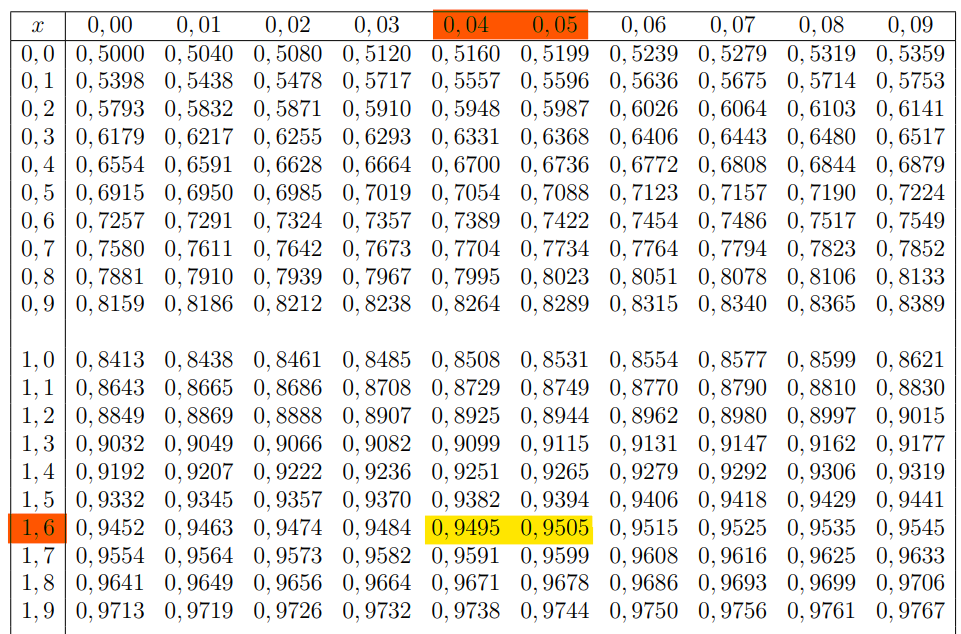
\includegraphics[width = \textwidth]{images/table_1.png}
\end{figure}

Ainsi si on revient à notre seuil $M$, il vérifie :
    $$\frac{M-\mu}{\sigma} = 1,645$$
    $$\Rightarrow M = \sigma \times 1,645 + \mu = 5 \times 1,645 + 22 = 30, 225$$
    
    \item Ici on cherche un intervalle de confiance à 95\% pour notre variable $Y$, i.e. on cherche une valeur $a$ telle que $$\P(\mu-a < Y < \mu +a) = 0,95$$
    
    Comme d'habitude, commençons par nous ramener à la loi centrée réduite :
    \begin{align*}
        \P(\mu-a < Y < \mu +a) &= \P(-a < Y-\mu < a)\\
        &= \P(-a/\sigma < Y_0 < a/\sigma)
    \end{align*}
    Le raisonnement sera similaire à la question 4, à la différence que l'on va utiliser une table différente que celle de la fonction de répartition de la loi centrée réduite. En effet, dans la question 4, on cherchait un intervalle de la forme $[M,+\infty[$, et on a vu que les calculs nous ont mené naturellement à la fonction de répartition. 
    
    Ici, on cherche un intervalle de la forme $[\mu-a,\mu+a]$, i.e. un intervalle centré sur la moyenne, et on peut remarquer, par symétrie de la loi normale autour de sa moyenne, que $$\P(-a/\sigma < Y_0 < a/\sigma) = \P(|Y_0|< a/\sigma) = 1 -\P(|Y_0|>a/\sigma)$$
    Cela nous incite donc à utiliser la table des valeurs extrêmes de la loi centrée réduite.
    
    \begin{remark}
        L'idée d'utiliser la table des valeurs extrêmes est souvent liée à la manipulation de notre loi normale dans un intervalle centré autour de sa moyenne.
    \end{remark}
    
    Ainsi :
    $$\P(\mu-a < Y < \mu +a) = 0,95 \Leftrightarrow  1 -\P(|Y_0|>a/\sigma) = 0,95 $$
    $$\Longrightarrow \P(|Y_0|>a/\sigma) = 0,05$$
    
    En utilisant la table des valeurs extrêmes, on trouve que $\P(|Y_0|>1,96) = 0,05$ d'où $$a/\sigma = 1,96 \Rightarrow a = 1, 96 \sigma$$
    
    En réinjectant cette valeur de $a$ dans notre intervalle, on peut écrire que l'intervalle de confiance recherché est $$[\mu-1,96 \sigma; \mu + 1,96 \sigma] = [22-1,96\times 5; 22+1,96\times 5] = [12,2\;;\;31,8]$$
    
    Cela signifie que 95\% des individus dégagent entre 12,2g et 31,8g de $\mbox{CO}_2$ par heure.
    
\end{enumerate}

\section*{Exercice 3}

Ici, on va étudier un temps de survie. On modélise souvent un tel phénomène par une loi exponentielle (cf. formulaire, diapos 10-11 du chapitre 2 ou partie 1.4.2 du polycopié pour les infos à retenir sur cette loi).
Notons donc $T \sim\mathcal{E}(\lambda)$ le temps de vie d'une cellule avant mutation, où $\lambda = 10^{-2} = 0,01$. 

\begin{enumerate}
    \item On définit la fonction de survie $S$ par $S:t\mapsto\P(T>t)$. Ainsi, $S(t)$ représente la probabilité pour une cellule de ne pas avoir mutée (en quelque sorte d'être toujours "vivante", d'où le nom de "fonction de survie") après $t$ jours. Explicitons cette fonction. Soit $t\ge 0$, la fonction de répartition de $T$ étant  $F_T(t) = \P(T\le t) = 1 - e^{-\lambda t}$:
    \begin{align*}
        S(t) &= \P(T>t)\\
        &= 1- \P(T\le t) \\
        &= 1 - (1 - e^{-\lambda t}) \\
        &= 1 - 1 + e^{-\lambda t})\\
        &= e^{-\lambda t}
    \end{align*}
    
    Enfin par définition de la loi exponentielle :
    $$\E(T) = \sigma(T) = \frac{1}{\lambda}= 100 \mbox{ jours}$$
    
    \item Calculons la probabilité demandée :
    \begin{align*}
        \P(T<40) &= F_T(40) \\
        &= 1- e^{-40.10^{-2}}\\
        &\approx 0,329
    \end{align*}
    
    Cela signifie qu'environ une cellule sur trois aura muté sous 40 jours.
    
    \item La médiane est, par définition, la valeur $M$ telle que $\P(T<M) = \P(T>M) = 0,5$. En particulier, $M$ vérifie $S(M) = 0,5$ d'après cette propriété. Résolvons cette équation :
    \begin{align*}
        S(M) = 0,5 &\Rightarrow e^{-\lambda M} = 0,5\\
        &\Rightarrow-\lambda M = \ln(0,5)\\
        &\Rightarrow M = -\frac{\ln(0,5)}{\lambda} \approx 69,3 \mbox{ jours}
    \end{align*}
    
    Cela signifie que la moitié des cellules vit plus de 69,3 jours et que l'autre moitié vit moins de 69,3 jours.
    
    \begin{remark}
        On aurait pu aussi faire le même raisonnement avec la fonction de répartition à la place de la fonction de survie, le résultat aurait été identique.
    \end{remark}
    
    \item Soient $\epsilon > 0$ et $t> 0$. Alors 
    \begin{align*}
        \P(T> t+\epsilon | T> t) = \frac{\P(\{T> t+\epsilon\}\cap \{T> t\})}{\P(T>t)}
    \end{align*}
    
    Or si $T>t+\epsilon$, alors $\epsilon$ étant positif, nécessairement $T>t$. Donc $\{T> t\}\subset \{T> t+\epsilon\}$, d'où :
        \begin{align*}
        \P(T> t+\epsilon | T> t) &= \frac{\P(T> t+\epsilon)}{\P(T>t)}\\
        &= \frac{S(t+\epsilon)}{S(t)}\\
        &=\frac{e^{-\lambda(t+\epsilon)}}{e^{-\lambda t}}\\
        &=e^{-\lambda(t+\epsilon)}e^{\lambda t}\\
        &=e^{\cancel{-\lambda t }-\lambda \epsilon +\cancel{\lambda t}}\\
        &=e^{-\lambda \epsilon} \\
        &= S(\epsilon) = \P(T>\epsilon)
    \end{align*}
    
    Le fait que 
    $$\forall \epsilon, t > 0, \; \P(T> t+\epsilon | T> t) = \P(T>\epsilon)$$
    est une propriété de toute loi exponentielle, et qui justifie l'utilisation de l'appellation "loi sans mémoire".
    
    En effet, regardons un exemple concret :
    \begin{itemize}
        \item $\P(T>40) = 1 - \P(T<40) = 1- 0,329 \approx 0,67$
        \item $\P(T>80) = S(80) = e^{-80.10^{-2}} \approx 0,45$
        \item $\P(T> 80 | T>40) = \frac{\P(T>80)}{\P(T>40)} = \frac{0,45}{0,67} \approx 0,67$
    \end{itemize}
    
    On a bien $\P(T> 80 | T>40) = \P(T>40)$
    
    La propriété "sans mémoire" de la loi exponentielle modélise une absence de vieillissement: que les cellules aient vécu 0 jour ou 40 jours, cela ne change pas la chance de muter au bout de 40 jours supplémentaires.
    
    \item Selon les observations :
    $$\P(T> 80 | T>40) < \P(T>40)$$
    Modéliser $T$ par une loi exponentielle semble donc ne pas être compatible avec les observations : $T$ n'est pas "sans mémoire".
    
    On peut en revanche modéliser $T$ par une loi de Weibull $\mathcal{W}(a,b)$ (cf.formulaire, diapos 12-14 du chapitre 2 ou partie 1.4.3 du polycopié pour les infos à retenir sur cette loi), puisque l'on observe une dégradation de la probabilité de survie au cours du temps, ce qui se modéliserait par une valeur $a > 1$.
    
\end{enumerate}


\end{document}
